\chapter{The Moral Side of Murder}

Michael Sandel opens this first lecture exactly where a course on justice ought to become uncomfortable: not with a definition, but with a case in which we are forced to choose before we know what principle we are choosing by. Following his order closely, and preserving the LazyLearn presentation curated by LazyingArt LLC, we move from a simple numerical contrast, to nearby variations that destabilize that contrast, to the emergence of two rival moral logics, and finally to Bentham, utility, and the harder problem of whether necessity, procedure, or consent can justify killing. The few formulas introduced below are editorial devices for making explicit the small arithmetic that the lecture repeatedly keeps before us; they are not formulas written in the lecture itself.

\section{Justice Begins with a Story}

We begin where Sandel begins: with a runaway trolley. The setup is deliberately spare. The trolley is moving too fast to stop, five workers are on the main track, and a side track contains one worker. The steering mechanism still works. The first question is not theoretical. It is immediate: what would we do?

\begin{figure}[h]
\centering
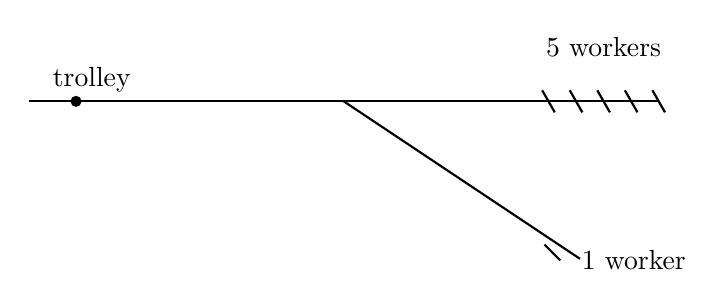
\begin{tikzpicture}[scale=1.0]
\draw[thick] (-4,0) -- (0,0) -- (4,0);
\draw[thick] (0,0) -- (3,-2);
\fill (-3.4,0) circle (2pt);
\node[above] at (-3.2,0) {trolley};
\foreach \x in {2.6,2.95,3.3,3.65,4.0} {
  \draw[thick] (\x-0.08,0.14) -- (\x+0.08,-0.14);
}
\node[above] at (3.3,0.45) {5 workers};
\draw[thick] (2.55,-1.82) -- (2.75,-2.02);
\node[right] at (2.9,-2.02) {1 worker};
\end{tikzpicture}
\end{figure}

The lecture's first poll reveals the simple arithmetic pressure built into the case. A small minority would continue straight; the overwhelming majority would turn. In editorial shorthand, the two available actions may be displayed as
\begin{align}
a_{\text{turn}} &: (N_{\text{die}},N_{\text{live}}) = (1,5), \\
a_{\text{straight}} &: (N_{\text{die}},N_{\text{live}}) = (5,1).
\end{align}
The point of the poll is not merely sociological. Sandel immediately asks for reasons. Why turn? The dominant answer is that it cannot be right to kill five when one could be killed instead. One student even extends the same style of reasoning to another tragic emergency: if fewer deaths can be chosen over more deaths, then the same principle seems to travel.

Already, then, the first moral maxim is on the table: better that one should die so that five should live.

\section{Trolley, Fat Man, and the Breakdown of a Simple Maxim}

Sandel's next move is exact and controlled. He does not abandon the one-versus-five structure. He alters a single structural feature. This time we are not the driver but an onlooker on a bridge. The trolley is again headed toward five workers. Beside us stands a large man whose body, if pushed onto the track, would stop the trolley and save the five.

The numerical structure appears unchanged:
\begin{align}
a_{\text{push}} &: (N_{\text{die}},N_{\text{live}}) = (1,5), \\
a_{\text{refrain}} &: (N_{\text{die}},N_{\text{live}}) = (5,1).
\end{align}
But the class reaction is no longer the same. Most who were willing to turn the trolley are unwilling to push the man.

\paragraph{Worked example.}
To isolate the pressure Sandel wants us to feel, it is useful to introduce a deliberately crude numerical proxy:
\begin{equation}
U_{\text{proxy}}(a) = N_{\text{live}} - N_{\text{die}}.
\end{equation}
On this stripped-down bookkeeping, the first two trolley cases look identical:
\begin{align}
U_{\text{proxy}}(a_{\text{turn}}) &= 5 - 1 = 4, &
U_{\text{proxy}}(a_{\text{straight}}) &= 1 - 5 = -4, \\
U_{\text{proxy}}(a_{\text{push}}) &= 5 - 1 = 4, &
U_{\text{proxy}}(a_{\text{refrain}}) &= 1 - 5 = -4.
\end{align}
If numbers alone settled the matter, the verdict should not change from the first case to the second. But it does change. That is the philosophical fact the lecture wants us to confront.

The ensuing discussion does not immediately yield a finished doctrine. Instead, it produces candidate distinctions. Perhaps pushing is worse because it is more active. Perhaps the man on the bridge was not already part of the danger. Perhaps steering a threat differs from using a person as the very instrument of rescue. Sandel then sharpens the difficulty by asking about a trap door: suppose the man could be dropped by turning a wheel rather than by using our hands. Even then, the class still feels the difference.

\subsection{Question \& Answer}

\paragraph{Question.} Why does turning the trolley seem permissible while pushing the fat man does not?

\paragraph{Answer.} The lecture does not offer a final theorem here, but it does produce a local clarification. The difference cannot lie simply in arithmetic, for the arithmetic is the same. Nor can it lie simply in bodily contact, since the trap-door variation preserves the sense that something has gone morally wrong even when no literal shove occurs. What survives the pressure of the exchange is a more general point: many of our judgments track not only outcomes but also the character of the act itself. In the first case we redirect a danger that is already in motion; in the second we make a person into the means by which the rescue is achieved. That distinction is still incomplete, but it is enough to propel the lecture toward a deeper contrast.

\section{Doctor, Triage, and Transplant}

The lecture now changes setting while keeping the formal pattern. We move from tracks and bridges to medicine. First comes emergency-room triage. Six patients arrive after an accident. Five are moderately injured; one is severely injured. If the doctor spends the day treating the one, the five die. If the doctor treats the five, the one dies.

Again the class largely follows the numbers. Treat the five.

Then comes a second medical case. A transplant surgeon has five patients, each in need of a different organ. A healthy man in the next room has all the needed organs. One could kill him and distribute the organs, saving the five.

The first medical case and the second have the same bare life-count:
\begin{align}
a_{\text{treat five}} &: (N_{\text{die}},N_{\text{live}}) = (1,5), \\
a_{\text{harvest}} &: (N_{\text{die}},N_{\text{live}}) = (1,5).
\end{align}
But once again the judgments diverge. Most will let the one severely injured patient die in order to save the five. Very few will kill the healthy patient for organs.

This repeated pattern is the real formal content of the opening lecture. Sandel is not yet building a moral theory from first principles. He is generating a data set of judgments by varying the case while holding the arithmetic roughly fixed. The lecture's method is comparative rather than deductive. We learn what our principles must explain by watching our own intuitions remain steady in some changes and collapse in others.

\section{Two Moral Logics Emerge}

At this point Sandel steps back and names what the class has already begun to reveal. It is useful to place the main cases side by side.

\begin{table}[h]
\centering
\[
\begin{array}{l|l|l|l}
\text{Case} & \text{Action favored by simple counting} & (N_{\text{die}},N_{\text{live}}) & \text{Dominant reaction} \\ \hline
\text{Trolley driver} & \text{Turn} & (1,5) & \text{Mostly permit} \\
\text{Bridge push} & \text{Push} & (1,5) & \text{Mostly reject} \\
\text{Emergency triage} & \text{Treat five} & (1,5) & \text{Mostly permit} \\
\text{Transplant surgeon} & \text{Harvest} & (1,5) & \text{Mostly reject} \\
\text{Dudley-Stevens defense} & \text{Kill one to save three} & (1,3) & \text{Mostly reject}
\end{array}
\]
\end{table}

\begin{definition}
Consequentialist moral reasoning locates the morality of an act in its consequences, that is, in the state of the world resulting from what we do.
\end{definition}

\begin{definition}
Categorical moral reasoning locates morality in duties, rights, or restrictions that hold regardless of consequences.
\end{definition}

The lecture arrives at these definitions from below. The first line of reasoning says: if five can live rather than die, that fact should govern the choice. The second line says: no, there are some things we must not do, even for the sake of a numerically better result. Sandel does not yet defend one side against the other. He extracts them from the discussion and names the contrast. The cases have done their work.

He also makes clear that these are not merely classroom puzzles. The two most influential thinkers attached to the opposing poles of the course are already named: Bentham on the consequentialist side, Kant on the categorical side.

\section{Why Philosophy Matters, and Why It Disturbs}

Before the lecture turns to Bentham in a more systematic way, Sandel widens the frame. The course will read great books, but not in order to leave them sealed off from ordinary life. The books are to be brought into contact with contemporary controversies: equality and inequality, affirmative action, free speech and hate speech, same-sex marriage, military service, and other disputes in which philosophy is already operating whether or not we acknowledge it.

The warning follows immediately. Philosophy does not simply furnish us with new information. It makes the familiar strange. That is why the toy cases at the start of the lecture are not disposable warm-ups. They are miniature demonstrations of what philosophy does: it takes an intuitive response from an unquestioned setting, turns it slightly, and makes us see that we no longer know what we thought we knew.

Sandel emphasizes two risks.

\begin{itemize}
\item The personal risk: once a familiar moral understanding has been unsettled, it cannot simply be returned to its earlier innocence.
\item The political risk: philosophical reflection may initially distance us from settled conventions and inherited civic habits rather than making us more practically effective.
\end{itemize}

The characteristic temptation, once these risks appear, is skepticism: perhaps each of us simply has a view, and perhaps there is no point in trying to reason further. Sandel resists this evasion. The persistence of moral disagreement is not proof that moral reflection is useless. On the contrary, it may show that these questions are unavoidable, because we live some answer to them every day whether we articulate that answer or not.

The aim of the course, then, is not to promise a painless consensus. It is to awaken what Sandel calls the restlessness of reason.

\section{Bentham, Utility, and the Return to Method}

After the internal break, the lecture resumes by restating the method that has been implicit from the beginning. Sandel now says openly what the first half has been doing.

\begin{enumerate}
\item We begin with judgments about particular cases.
\item We try to articulate the principles behind those judgments.
\item We confront those principles with new cases.
\item We revise judgments and principles in light of one another until they can stand together.
\end{enumerate}

Only after this methodological recap does Bentham enter as a systematic thinker. The central utilitarian thought is simple enough to be stated in ordinary language and, cautiously, in editorial notation. Let \(H(a)\) denote the happiness resulting from act \(a\), and let \(S(a)\) denote the suffering resulting from it. Then the lecture's statement of utility may be compactly written as
\begin{equation}
U(a) = H(a) - S(a).
\end{equation}
Sandel gives the content of this expression in words:
\begin{align}
\text{utility} &= \text{pleasure} - \text{pain}, \\
               &= \text{happiness} - \text{suffering}.
\end{align}
The utilitarian directive then becomes
\begin{equation}
a^\ast = \underset{a}{\mathrm{arg\,max}}\; U(a).
\end{equation}

\begin{remark}
These formulas are editorial shorthand for Sandel's presentation of Bentham. The lecture itself states the view in prose: the right act, and the just law, is the one that maximizes the overall balance of happiness over suffering.
\end{remark}

Bentham's route to the principle matters. He begins with the claim that human beings are governed by two sovereign masters, pain and pleasure. Since we seek pleasure and avoid pain, morality and legislation should be organized around that fact. In its most compressed public slogan, utilitarianism becomes the greatest good for the greatest number. If one wants one more symbolic compression, the slogan may be written as
\begin{equation}
a^\ast = \underset{a}{\mathrm{arg\,max}}\; \sum_i u_i(a),
\end{equation}
but the lecture's point is not formal machinery. The point is that Bentham offers a clear theory of the intuition already visible in the trolley case: outcomes matter, and the right action is the one that brings about the best aggregate state of the world.

\section{Dudley and Stevens: Necessity, Lottery, and Consent}

Sandel now asks utilitarian reasoning to leave the safety of classroom hypotheticals and enter a real case: \emph{The Queen v. Dudley and Stephens}. Four men are cast adrift after a shipwreck. Food is minimal, fresh water absent, rescue nowhere in sight. Richard Parker, the cabin boy, becomes ill after drinking sea water and appears close to death. Dudley proposes a lottery. Brooks refuses. No lots are drawn. The next day Dudley kills Parker with a penknife. The survivors live by consuming his body and blood until rescue arrives.

The defense is plain: necessity. Better that one should die so that three could survive. In the most compressed form of the defense, the case is represented as
\begin{equation}
a_{\text{kill Parker}} : (N_{\text{die}},N_{\text{live}}) = (1,3).
\end{equation}
But even here the lecture does not let the arithmetic stand alone. Unlike the trolley case, the alternative outcome is not cleanly known in advance. Rescue may come soon or late. The defense therefore quietly imports a conjecture about consequences:
\begin{equation}
U(a_{\text{kill Parker}}) \stackrel{?}{>} U(a_{\text{wait}}).
\end{equation}
Some students then enlarge the calculation in a Benthamite direction. It is not merely three lives against one. The three survivors have families, dependents, and wider effects back home, whereas Parker is an orphan. The welfare calculus may therefore appear stronger than the head-count alone suggests.

Yet the majority of the class still resists. Some say that no circumstance authorizes us to take another person's life into our own hands. Others insist that murder remains murder, even when necessity and aggregate benefit are invoked. Still others begin to search for a middle path: perhaps the real problem is not killing as such, but the absence of a fair procedure or the absence of consent.

\subsection{Question \& Answer}

\paragraph{Question.} Would a lottery, or Parker's consent, make the killing morally permissible?

\paragraph{Answer.} The lecture develops three distinct possibilities and refuses to collapse them into one.

\begin{enumerate}
\item \textbf{Necessity and utility.} On this view, desperate circumstances and aggregate survival can justify the sacrifice. This is the strongest consequentialist reading of the case.
\item \textbf{Fair procedure.} Some students argue that the absence of consultation is what makes the act intolerable. A lottery would count everyone equally and remove the unilateral judgment that one life simply matters less than the others.
\item \textbf{Consent.} Others push further: if Parker himself freely agreed, then the moral status of the killing might change because agency would shift from imposed sacrifice to accepted sacrifice.
\end{enumerate}

But the lecture also shows why these modifiers do not end the argument. Critics reply that consent under such conditions may be coerced, that a lottery may still deliver an unjust outcome, and that even if a person may sacrifice himself, it does not follow that another may kill him. The categorical objection therefore survives all three modifications. Murder, on this view, is still murder.

Sandel ends the case not with a verdict but with three questions that launch the rest of the course.

\begin{enumerate}
\item If killing is categorically wrong, is that because persons have rights that cannot be reduced to welfare?
\item Why should agreement to a fair procedure justify whatever outcome the procedure yields?
\item What moral work does consent do, and why does it seem to transform the status of an act that would otherwise be wrong?
\end{enumerate}

These questions are the real terminus of the lecture. The case of Dudley and Stephens is not merely another example. It is the point at which the opening intuitions, Bentham's theory, and the stubborn appeal of categorical constraints are forced into the same frame.

\section{Summary}

This first lecture establishes the method and the stakes of the course. We begin with judgments under pressure, extract the principles those judgments seem to presuppose, and then discover that those principles fracture under carefully chosen variations. Out of the trolley, bridge, doctor, and transplant cases there emerges the contrast between consequentialist and categorical moral reasoning. Out of Bentham there emerges a systematic statement of the consequentialist side. And out of Dudley and Stephens there emerges the unresolved problem that will drive the next stage of inquiry: whether the claims of welfare can ever override rights, whether fair procedure can justify sacrifice, and what, precisely, consent changes.